\documentclass{article}
\usepackage{blindtext, graphicx}
\usepackage{amsmath}
\usepackage{verbatim}
\usepackage{hyperref}
\usepackage[margin=1in]{geometry}
\usepackage{parskip}

\usepackage{float}

\begin{document}
%
% paper title
% can use linebreaks \\ within to get better formatting as desired
\title{CS 143: Final Report}


% author names and affiliations
% use a multiple column layout for up to three different
% affiliations
\author{{Rafael Fueyo-Gomez}
\and
{Cortland Perry}
\and
{Kelsi Riley}
\and
{Sakthi Vetrivel}}
\maketitle
\section{Introduction}

For our term project, our team decided to pursue the network simulator. At a high level, the simulator takes in a input of a the description of network, such as its hosts, routers, links, and flows, runs a simulation for a user-specified duration, and outputs graph demonstrating the progression of certain metrics, such as flow rate, window size, or buffer occupancy, after the end of the run. 

This simulator is written in Python3 and makes use of the matplotlib package. Code can be found at \url{https://github.com/rafugo/cs143_simulator}. Instructions to run the test cases can be found in the repository's README file.

\section{Simulator Architecture}

\subsection{Simulator Class}

Our simulator class contains all of the network objects needed to simulate our network. 

\begin{description}
	\item[$\bullet$ \_\_init\_\_(self, string filename)] This function uses the input file specified in filename to create network objects based on a network description.
	\item[$\bullet$ plot\_metrics(self)] This function uses all of the metrics that were recorded during simulation and plots them. The graphs are then outputted as png files in the directory of the code.
	\item[$\bullet$ run(self)] This function runs the actual simulator. Upon starting the simulator, we first have all of router make their handshakes to learn the routing table for the network. Then, we run all network events on a timestep basis. So, for a user-specified amount of time, we run the simulator for so many timesteps. For every timestep, we make calls to link class to try to send all packets in the buffer, and calls to every flow to send packets in the flow. We then increment our global clock. Moreover, every five seconds, we send all of our link states throughout the router to update the link states and the routing table if needed.
	% Maybe we need to explain more about the timesteps here?

\end{description}


\subsection{Packet Class}

\begin{description}
	\item [$\bullet$ \_\_init\_\_(self, int sourceid, int flowid, int destinationid, int packetid, string packet\_type, string data = '')] Initialize a packet object. sourceid referes to the id of the source (whether it's a router or a host). flowid refers to the id of the flow the packet belongs to. destinationid referes to the id of the destination (whether it's a router or a host). packetid is the identification of the packet within the flow and is its number in the sequence. packet\_type is the type of the packet and can take on the values of STANDARDPACKET: a normal packet, ACKPACKET: an acknowledgement packet, ROUTINGPACKET: a routing table packet, SYNPACKET: a synchronization packet, SYNACK: a synchronization packet acknowledgement. 
\end{description}

\subsection{Host Class}

Our host class simulates the behavior of a host in our network.

\begin{description}
	\item [$\bullet$ \_\_init\_\_(self, int hostid, int linkid)] Initializes a host object. The hostid allows us to identify against different host objects and the linkid allows to identify which link is associated with this host.
	\item [$\bullet$ send\_packet(self, Packet p)] Send the packet p by adding (or attempting to add) the packet to the link buffer.
	\item [$\bullet$ receive\_packet(self, Packet p, int linkid)] Sends acknowledgements of packets received and notifies the correct flow of these acknowledgements.
\end{description}

\subsection{Router Class}

\begin{description}
	\item [$\bullet$ \_\_init\_\_(self, int id, List<Link> links)] Initializes a router object. The id allows us to identify different routers, and the list of links refers to the links that are connected to this router object. 
	\item [$\bullet$ receive\_packet(self, Packet packet, int linkid)]  Processes packets and has case handling for the different packets it might receive such as handshake packets, handshake acknowledgements, standard packets or routing packets. 
	\item [$\bullet$ forward\_packet(self, Packet packet)] Forwards packets based on the routing table and their destination.
	\item [$\bullet$ send\_handshake(self)] Send the initial handshake packet to the adjacent routers to determine which nodes are connected.
	\item [$\bullet$ recalc\_link\_state(self)] Recalculates the link states.
	\item [$\bullet$ send\_link\_state(self)] Send out our link state array to neighbors.
	\item [$\bullet$ receive\_handshake\_ack(self, Packet packet, int linkid)] Processes handshake acknowledgement.
	\item [$\bullet$ receive\_link\_state(self, string array  state\_array\_actual)] Upon receiving a link state, the router updates its own link state array.
	\item [$\bullet$ run\_dijkstra(self)] Run's Dijkstra's algorithm to determine the routing table.
\end{description}


\subsection{Link Class}
\begin{description}
	\item [$\bullet$ \_\_init\_\_(self, int linkid, int connection1, int connection2, float rate, float delay, int buffersize, bool track1=True, bool track2=True)] Initializes a link object for our network. linkid is the ID for this link object. connection1 and connection2 are the id's of the hosts/routers at the ends of the link. rate and delay are floats that refer to the rate and propagation delay of the link. buffersize is the size of the buffer for this link. track1 and track2 are boolean values to determine if we should track metrics for this link. 
	\item [$\bullet$ add\_to\_buffer(self, Packet packet, int sender)] Add packet to buffer based on the sender of the packet.
	\item [$\bullet$ send\_packet(self)] Tries to send a packet on both of the half links corresponding to the link.
	\item [$\bullet$ HalfLink] Represents one direction of the Link. (i.e. all packets traveling across a given HalfLink will be going to the same destination) Class has its own definitions for add\_to\_buffer and send\_packet.
	
\end{description}

\section{Congestion Control}

Our congestion control takes place in our flow class. For our project, we've implemented two congestion control algorithms, TCP Reno and TCP Fast. To do this, we have two different Flow classes (flow\_reno.py and flow\_fast.py), with different implementations of the same public methods. Here's an overview of all of the public methods. 

\begin{description}
	\item [$\bullet$ run(self)] This function is called at every timestep by the simulator for the flow to send any packets as necessary for that timestep.
	\item [$\bullet$ process\_ack(self, Packet p)] Process an acknowledgement once it's received by a host. Checks for duplicate acknowledgements and changes congestion control states, window size, and threshold accordingly.
	\item [$\bullet$ send\_packets(self)] Send the packets for the flow depending on the current system time and the acknowledgements that have been received thus far.
\end{description}

\subsection{TCP Reno}

In our TCP Reno implementation, we have three possible states for the algorithm to be in: slow start, congestion avoidance, or fast recovery. Dependent on these states, we have different behavior. If we are in the slow start state of our algorithm, for every acknowledgement that is not a duplicate acknowledgement received, we increase our window size by one. If we are in the congestion avoidance state, we increase our window size by $\frac{1}{cwnd}$ where $cwnd$ is the current window size. If we are in fast recovery, we do not send any packets until the retransmission of the dropped packet is successful. We then half our window size and enter congestion avoidance.

To start, our window size is initialized at 1 packet. Our window start, which refers to the first packet in the next window of consecutive packets to be sent, starts at 0. The congestion control algorithm starts in the slow start state with a slow start threshold of 1000. We chose this initial value to be arbitrarily large, so the network will either timeout or receive three duplicate acknowledgements before it enters congestion avoidance for the first time. Before we start sending any packets from our flow, we send a synchronization packet. We then wait for this packet to return and be acknowledged to calculate our initial RTT value.

To send packets for our flow, at every timestep, we see if there are any packets in our current window that have not yet been sent, and if there are, we send them. To keep track of duplicate acknowledgements, we have a counter for consecutive duplicate acknowledgements. Once we reach three, we enter fast retransmit and fast recovery. 

Morever, to calculate the round trip time for our packets, we use Karn's algorithm, which states that the round trip time calculation is only based on packets that are sent and acknowledged only once. All other packets are ignored in the metric. To keep track of round trip times, we have a dictionary send\_times as an attribute of the flow\_reno class. This maps packet IDs to the time at which they were last attempted to be sent. This dictionary only includes packets that have been sent but not yet acknowledged. Likewise, we have a dictionary dup\_count that maps packet ids to the number of times they have been sent. So if a packet has a dup\_count larger than 1, then we do not consider it in the calculation of the round trip time. Thus, every time we process an acknowledgment, we check the dup\_count of the packet that is acknowledged, and then access its send\_time to calculate the latest RTT. 

For packet timeouts, we use a timeout marker. This timeout marker is based on the last non-duplicate acknowledgement received and an RTO value. This RTO value is calculated as $2 \times RTT$. Thus, every time an acknowledgement is processed, the timeout marker is reset to be the current system time $+$ RTO. Then, at every time step, we check if we have passed this timeout marker, meaning a packet has timed out -- specifically the first packet that we have sent but have not received an acknowledgement for. Upon recognizing a packet timeout, we set our slow start threshold to half of the current window size and set our window size to 1 and enter the slow start state. We also retransmit the lost packet and then double the RTO for future timeouts. Additionally, to avoid entering a loop where packets timeout repeatedly, resulting in overpenalizing the network for dropping packets, we keep track of a next\_cut\_time. This variable refers to the next time that cut our threshold in half and ensures that we wait 1 RTO before cutting the threshold again. 

\subsection{TCP FAST}

In our TCP FAST implementation, we also have three possible states for the algorithm to be in: slow start, congestion avoidance, or fast recovery. The way TCP FAST works, it is not so much dependent on ACKs to modify its state, but moreso on the RTT.

In the slow start state, we increment the window size by one for every ACK, similar to in Reno. However, we limit this behavior to every other RTT. That is, we have an active RTT and a frozen RTT. During the "active" RTT, we increment the window size and during the "frozen" one, we do not do anything. Our implementation then exits slow start and enters congestion avoidance when it thinks that it is approaching the estimated throughput. It also may exit slow start when there are three duplicate ACKs, and then enters fast recovery.

To calculate when we may be nearing our estimated throughput, we do a simple estimate. We keep track of how many packets we receive during each frozen RTT (in reality, just the current and the previous frozen RTTs). Thus, we have the given throughput of an RTT as $\frac{m_{current}}{RTT}$ with $m_{current}$ being the amount of packets received in the current frozen RTT. Note that, since we are doubling the window size every other RTT, we should expect $$\frac{2 * m_{previous}}{RTT_{previous}} = \frac{m_{current}}{RTT_{current}} \Rightarrow \frac{2 * m_{previous} * RTT_{current}}{RTT_{previous}} = m_{current}$$
If we receive $90\%$ less than the predicted $m_{current}$, then we believe to be increasing the buffer size in the bottleneck link along the path, so we go into congestion avoidance in order to avoid dropping packets. We chose $90\%$ in order to be conservative and not drop any packets by being too aggressive.

We enter fast recovery in the same way we would enter it in Reno, and it is handled exactly the same way. Duplicate ACKs are also handled the same as in Reno.

Once we enter congestion avoidance, we continue with the alternating active and frozen RTTs. Every time we enter a new active RTT, we set a goal window size that we want our window size to be by the end of the active RTT. This goal window size is whatever the "next window size" is at that given moment. The next window size is updated every 20 ms, according to the following equation: $$ w \leftarrow \textrm{min}(2w, (1-\gamma)w + \gamma(\frac{\textrm{baseRTT}}{\textrm{RTT}}w + \alpha)) $$
where $w$ on the right hand side is the current window and the $w$ on the left hand side is the next window size. We chose $\alpha = 15$ and $\gamma = 0.5$. 

For our RTTs, we used the same algorithm as in Reno. We also followed the same timeout procedure.


\section{Metrics Tracking}

To track metrics during our simulation, we created a global dictionary with string keys of the form {\em object : metric}, where {\em object} is the ID of the specific object that the dictionary is tracking, which will be a flow, link, half-link or host and {\em metric} is the metric that the dictionary is tracking. Each of these keys maps o a value of another dictionary, where the dictionary mapped to contains items of the form (time, value), where the time is the key, and the value is the value for that metric at that time. In our simulation, we also kept track of which objects we would be tracking statistics for and we would only add entries to our global dictionary of statistics corresponding to those being tracked. This served to save both time and space, so our simulation wouldn't spend time computing and storing values we didn't intend to use. 

\subsection{Link Statistics}
The only metric we ended up tracking at the link level was the number of dropped packets, for links that we track metrics for, we track packet loss for both directions of the link.
\subsubsection{Dropped Packets}
To track packet loss along links, we added a field droppedpackets to the Link class. Then, when any network object tries to add a packet to either buffer associated with a link, the link checks if the packet was dropped, and if it was, increments the value stored in droppedpackets. Then, at each time step of the simulation, each link calls update\_link\_statistics(), which adds the current value of droppedpackets to the dictionary with key value which is the current time of the global clock and then resets the value of droppedpackets to be 0. Thus, each point in our packet loss graph corresponds to a single time step of the simulation and represents the number of packets dropped during that time step. 

\subsection{HalfLink Statistics}
We tracked both link rate and buffer occupancy at the half-link level so that we could really focus on the behavior of the link in the direction of interest. 

\subsubsection{Link Rate}
To track the link rate of a half-link we added a couple fields to the HalfLink class, {\em lrwindow} and {\em lrsteps}. {\em lrwindow} stores the window of time over which we are computing the link rate for, and is a multiple of the size of a time step. Then {\em lrsteps} stores a list of values corresponding to each time step in the window, where each value indicates the amount of data transmitted by the link in the corresponding time step in bits. All of the link rate tracking occurs in the  send\_packet() function, which updates these values and computes the current estimate for rate by taking the sum of all the values in {\em lrsteps} and dividing them by the minimum of the amount of time that has passed and {\em lrwindow}. Then, if we add the estimated rate to the corresponding dictionary with a key of the current time of the global clock. 

\subsubsection{Buffer Occupancy}
Each half-link stores {\em buffersize} and {\em buffercapacity}, which store the current occupancy of the buffer and its capacity, respectively. As packets are added and removed from the buffer, {\em buffersize} is updated accordingly. The half-link calls update\_link\_statistics() at each times step, which then adds {\em buffersize} as a value to the corresponding dictionary with a key value that is the current time. 

\subsection{Flow Statistics}
For each flow which the simulator is tracking, window size, flow rate, and flow round trip time (RTT) were tracked. All flow statistics are only updated if {\em done} is false and if the current time is greater than or equal to the flow's start time. This ensures that we only track flows once they have started and while they are still active. Flows call update\_flow\_statistics() at each time step to update these statistics. 

\subsubsection{Window Size} 
When update\_flow\_statistics() is called, the current window size of the flow, which is updated and managed by the congestion control for the flow, is added to the dictionary corresponding to this flow's window size with a key value that is the current time. 

\subsubsection{Flow Rate}
To track the flow rate, {\em frwindow}, {\em frsteps} and {\em added} were added to the Flow class.  {\em frwindow} stores the window of time over which we are computing the flow rate for, and is a multiple of the size of a time step. Then {\em frsteps} stores a list of values corresponding to each time step in the window, where each value indicates the amount of data for which we received a new acknowledgment in the corresponding time step in bits. Because the flow will only be able to receive at most one ACK per time step in our simulation (due to the link rates which we are calibrated for, size of ACK packets, and size of our time step), each value in this list will be either 0 or the size of a packet in bits. {\em added} is a boolean value which indicates whether or not we have already added a value to {\em frsteps} on a given time step. 

When the flow receives an ACK packet p, it calls track\_metrics(p), which checks if the packet being acknowledged by has already been acknowledged. If so, it does nothing. Otherwise, it updates the dictionary storing successfully transmitted packets to show that the packet being acknowledged was successfully transmitted, appends the size of a packet in bits to {\em frsteps} and sets {\em added} to be true. 

The flow calls update\_flow\_statistics() at every time step. If {\em added} is false, 0  is appended to {\em frsteps}. If {\em frsteps} is has fewer or as many elements as time steps which {\em frwindow} covers, the rate is computed as the sum of its elements divided by the amount of time for which the flow has been flowing. Otherwise, we remove its first element and compute the rate as the sum of its elements divided by the window size. Then, the computed rate is added to the dictionary corresponding to the flow's flow rate with a key of the current time of the global clock.

\subsubsection{Flow RTT}
The first time the flow sets its RTT, it sets {\em setRTT} to be true and adds the current RTT to the dictionary corresponding to its RTT with a key that is the current time. When update\_flow\_statistics() is called and {\em setRTT} is true, the current RTT of the flow, which is updated and managed by the congestion control for the flow, is added to the dictionary corresponding to this flow's RTT with a key value that is the current time. 

\subsection{Host Statistics}
\subsubsection{Host Flow Rate}


\section{Results}

\subsection{Test Case 2}

\subsubsection{TCP Reno}

Run using \textbf{python3 main.py test\_case2\_reno.json 70}.

\begin{figure}[H]
\centering
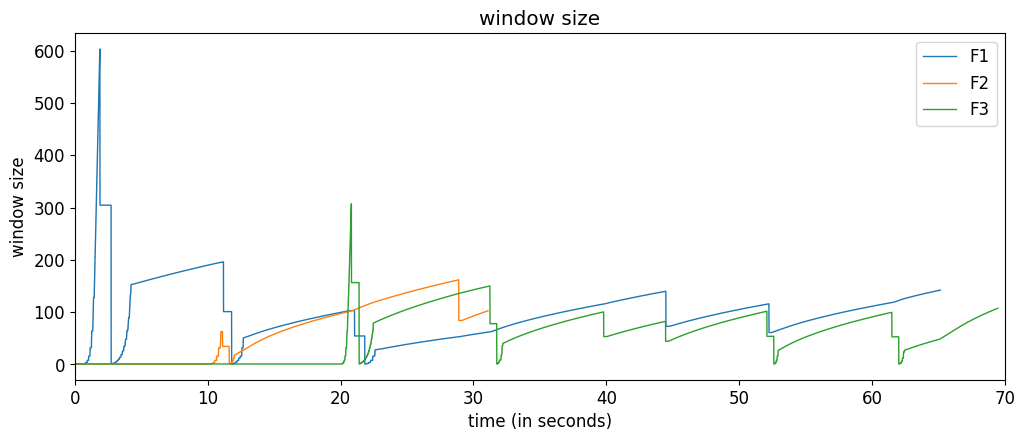
\includegraphics[width = \textwidth]{test_case2_reno window size.png}
\end{figure}

Initially, since we are running Reno, we have a very aggressive start to Flow 1 window size, resulting in 3 duplicate ACKs, fast recovery, and eventually timeout. Our congestion avoidance works well, starting at the threshold at around half + 3 of the window size. At around 10 seconds, Flow 2 enters the system aggressively and causes the loss of packets, timing out both Flow 1 and Flow 2 after fast recovery fails. Flow 1 congestion avoidance triggers at a higher window size than Flow 2 because of how the thresholds were set. At around 20 seconds, Flow 3 enters aggressively and causes link 3 to congest and packet loss for both itself and Flow 1. Flow 2 remains not only unscathed, but has an increase in RTT (due to Flow 1 timing out) and thus increments its window size quicker momentarily. Since Flow 1 has a significantly higher RTT than Flow 2 and Flow 3, it takes longer to get to its threshold. Flow 3 is more aggressive because of its smaller RTT and thus it grows to a higher window size. In addition, the bottleneck at this point is both in link 1 and link 3, so Flow 1 remains at a smaller window size until 30 seconds in. At 30 seconds in, Flow 2 dies off, leaving Flow 1 with just one bottleneck at link 3. Coincidentally, Flow 3 drops a packet around that time, and Flow 1 takes advantage of increased RTT due to lowered buffer occupancy contribution from Flow 3. 

Here the system enters an interesting scenario where it seems like if a packet is dropped, it is only from Flow 3 and not Flow 1. We believe that this is due to our implementation of the underlying links. The links are ordered by priority, albeit not intentionally. Our implementation fires off each link one at a time. Link 2 will be fired before link 6, and thus if the buffer is too full for link 6 to put all the packets it can in the buffer, then it will drop packets. Thus, Flow 1 will not experience packet loss while Flow 3 will. Therefore, we believe that if the links were given equal priority when it comes to which sends packets first, we would have a more similar graph to that in the sample traces.

\begin{figure}[H]
\centering
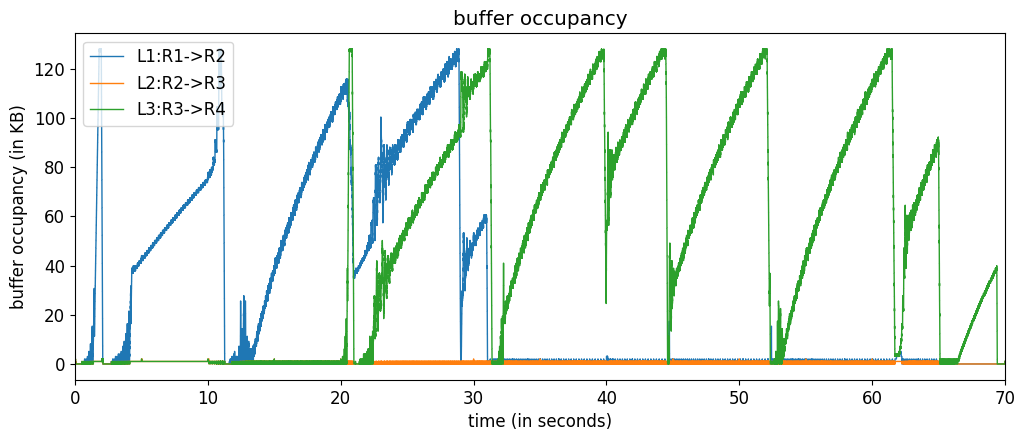
\includegraphics[width = \textwidth]{test_case2_reno buffer occupancy.png}
\end{figure}

The buffer occupancy closely mirrors our window sizes. As window size increases, the buffer occupancy increases. Note the spikes at 0, 10, and 20 seconds as flows enter and exit the system. This is due to window sizes exponentiating. At 30 seconds we see that there is a quick increase in the buffer occupancy for L3.

\begin{figure}[H]
\centering
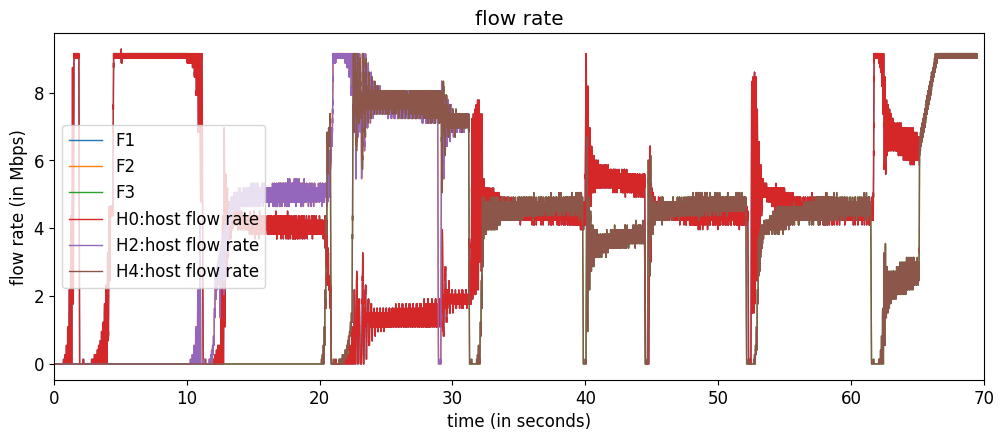
\includegraphics[width = \textwidth]{test_case2_reno flow rate.png}
\end{figure}

The flow rate caps out initially for link 1, because it is the bottleneck. At 10 seconds, when Flow 2 enters the system, it becomes a tighter bottleneck since both Flow 1 and 2 are using link 1. Thus, the flow rates drop. The flow rate for Flow 2 is faster due to smaller RTT, even if the window size is smaller. At 20 seconds, Flow 3 enters the system. It first crashes the Flow for Flow 1 and 3, but then creates a bottleneck at link 2 for Flow 1. At this moment, Flow 2 and Flow 3 have the same flow rate, while Flow 1 experiences a lower rate. At 30 seconds, Flow 2 dies off and then Flow 1 and Flow 3 share the same bottleneck and equilibrate flows.  Over time, the flows have to re-equilibrate due to Flow 3 dropping packets and also general congestion avoidance/fast recovery interactions.

\begin{figure}[H]
\centering
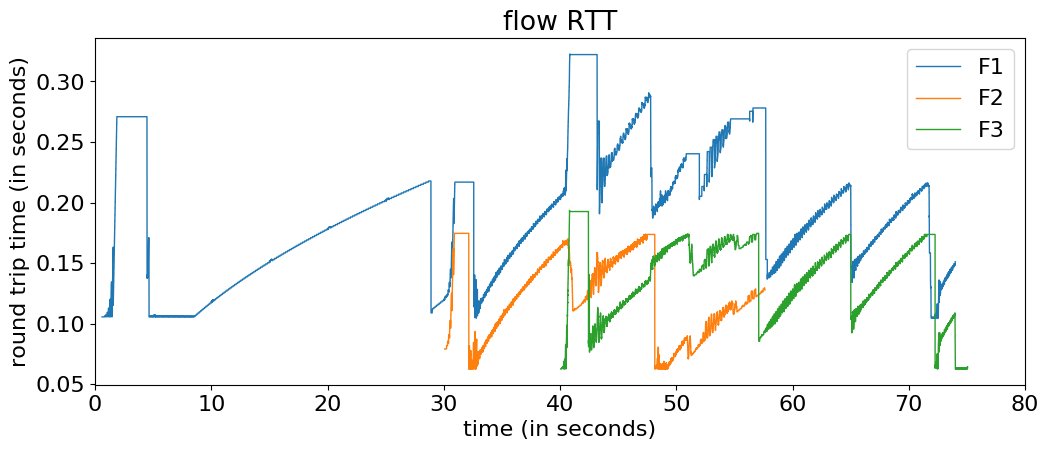
\includegraphics[width = \textwidth]{test_case2_reno flow RTT.png}
\end{figure}

This obviously mirrors the buffer occupancy. As the occupancy goes up, the queueing delay increases and thus the RTT increases.

\begin{figure}[H]
\centering
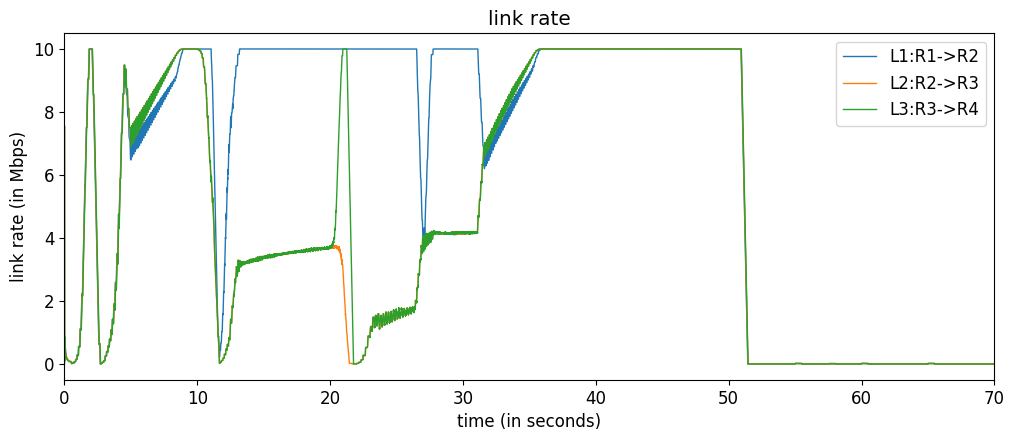
\includegraphics[width = \textwidth]{test_case2_reno link rate.png}
\end{figure}

Initially, we cap out the link rate for all the links (cannot be seen as link 3 takes priority in the graph). At around 10 seconds, Flow 2 enters and causes packet loss, dropping the link rates. As we re-equilibrate, we have that link 1 is the bottleneck, so the other links experience lower rates. Around 20 seconds, Flow 3 enters and after the packet loss events, link 1 and link 3 are the new bottlenecks, with link 2 being smaller because of that. Thus, they are maxed out while link 2 sits low. At 30 seconds, Flow 2 exits the system and then link 3 is the only bottleneck, so it remains maxed out. Meanwhile, link 1 and 2 experience the effects of the congestion avoidance/fast recovery. The reason for link 2's rate being higher than link 1's rate is that, since there were already packets in the buffer for link 2, when the system re-equilibrates, those packets have an influence and thus cause the link rate to be higher in general. At the end, link rate 3 drops slightly as Flow 1 exits, and then recuperates as Flow 3 ups its window size and output.

\begin{figure}[H]
\centering
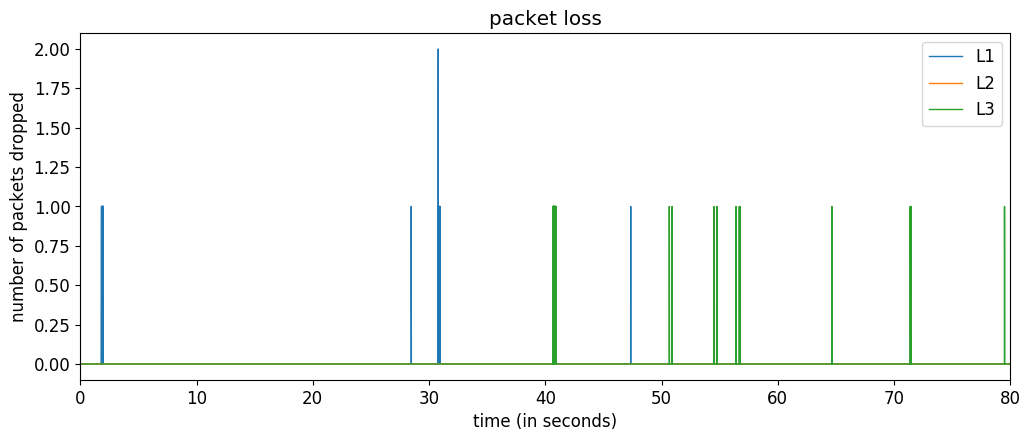
\includegraphics[width = \textwidth]{test_case2_reno packet loss.png}
\end{figure}

This matches up with the timeouts we experience, as well as the entries into fast recovery, across all the flows.

\subsubsection{TCP Fast}

Run using \textbf{python3 main.py test\_case2\_fast.json 70}.

\begin{figure}[H]
\centering
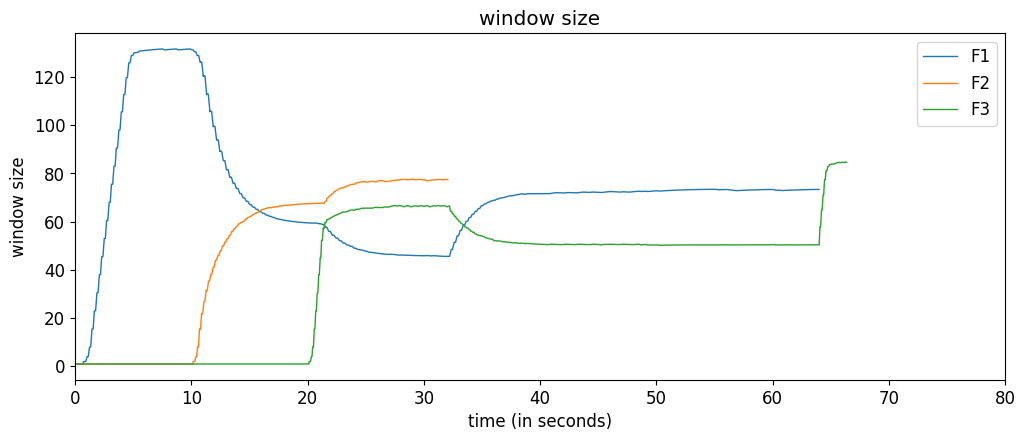
\includegraphics[width = \textwidth]{test_case2_fast window size.png}
\end{figure}

Here we have the window size graph of our flow for TCP fast. Looking at three critical points, 0, 10, and 20 seconds, where each flow starts. Each flow initially starts in the fast slow start state, which causes each flow to increase its window size until the throughput that the flow is using in the last round trip time is less than 90 percent of the expected throughput. At that point, each of our flows enters congestion control and reaches equilibrium. Then, when the next flow starts, our equilibrium window size will lower in order to adjust to the window size that the new flow is contributing.

\begin{figure}[H]
\centering
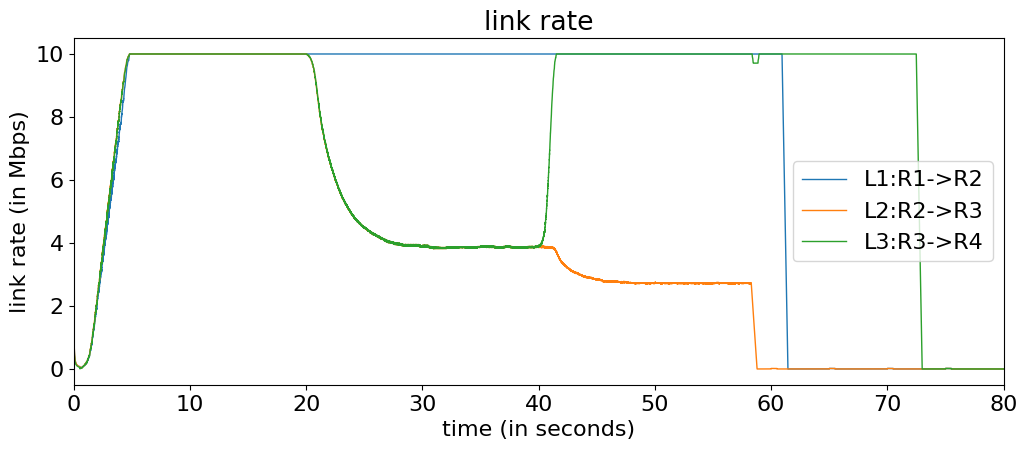
\includegraphics[width = \textwidth]{test_case2_fast link rate.png}
\end{figure}

Here we have the link rate measurements of link 1, 2, and 3 in test case 2. Initially, we only have 1 flow using all three links, which means that all three links can be used to full capacity with the one flow. When our second flow enters, it is only using link 1, which then means that link 1 is going to be used to full capacity, whereas the flow rate of our first flow will be lowered, and thus will make the link rate of links 2 and 3 lower because they will not be used to their full potential. Then, when our third flow starts and all three flows are running simultaneously, we can see that link 1 and 3 are being used by two flows and thus will be used to their full capacity, whereas the second link will be used only by flow 1. Finally, when just flow 1 and flow 3 are active, we can see that link 3 is being used to full capacity. Link 1 and link 2 are only being used by flow 1, but when flow 2 died flow 1 sees link 2 as having some small amount of packets in the buffer, (because of how our links have priorities) which is why it will then be used slightly faster than link 1. The dip that occurs in link 3 at the very end occurs because when flow 1 finishes, flow 3 does not immediately realize that flow 1 is no longer sending packets, so it takes some time for it to increase its window size to use the link to full capacity.

\begin{figure}[H]
\centering
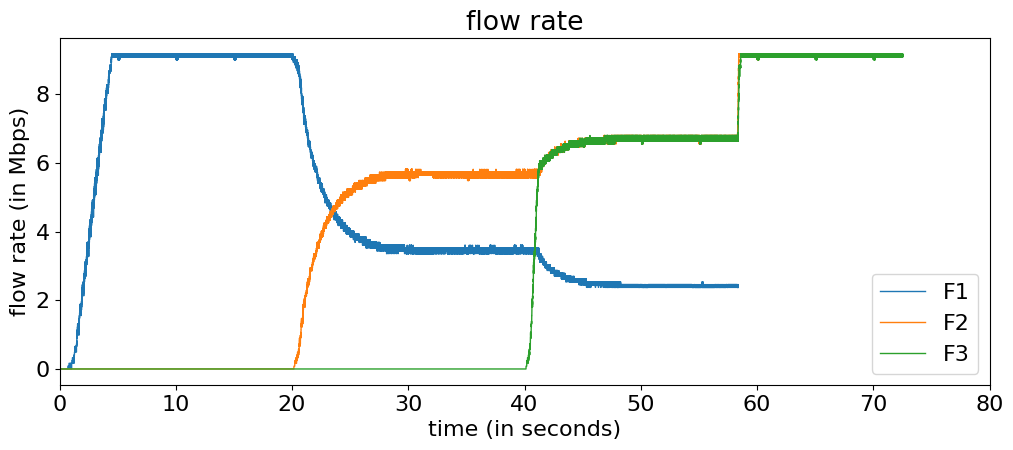
\includegraphics[width = \textwidth]{test_case2_fast flow rate.png}
\end{figure}

First, we will explain the flow rates seen in the graph, and then we will quantitatively explain the behavior some unexpected behavior that we observe. First, we can see that our flow rate for our first flow correctly utilizes the given links. Then, once our second flow emerges, both of our flows have to share link one, and thus the flow rates for both of them combine to the rate of where the bottleneck occurs. Then, when our third flow starts, we have two bottlenecks that our first flow has to go through, whereas there is only bottleneck for both flow 2 and 3 to transmit packets through (this can be slightly unexpected and will be quantitatively explained below). Thus, each of those will have a flow rate that twice that of flow 1. Finally, when flow 2 ends, flow 1 and flow 3 share the capacity of link 3, and thus their flow rate is the same as well. 

Note that in the flow rate for fast, we have unexplained behavior in which flow 2 has a larger rate than flow 1, and has the same flow rate as flow 3. 

We can explain this with the following derivation. First, we can model the throughput of our function using FAST for some flow i as: $ x_i = \frac{\alpha}{q_i} $

In the time in question, we see that flows 1 and 2 share L1, and flows 1 and 3 share L3, which then we know both become the bottleneck links. We then have $x_1 + x_2 = 10 $ and $x_1 + x_3 = 10 $. We know that L2 is underutilized, which means there are no queues on L2 and thus $p_2 = 0 $ where p is the queuing delay on link 2.

We know, based on our initial claim, $ x_2 = \frac{\alpha}{p_1} = \frac{\alpha}{p_3}  = x_3$

We also know, $x_1 = \frac{\alpha}{p_1 + p_2} = \frac{x_2}{ 2}$ because we know the queuing delay is the same on both $p_1 and p_2$ (because of how we defined the links).

Thus, we get a ratio between $x_1$ and $x_2$ of 1:2, which is what we see in the graphs and thus explains our interesting behavior.

\begin{figure}[H]
\centering
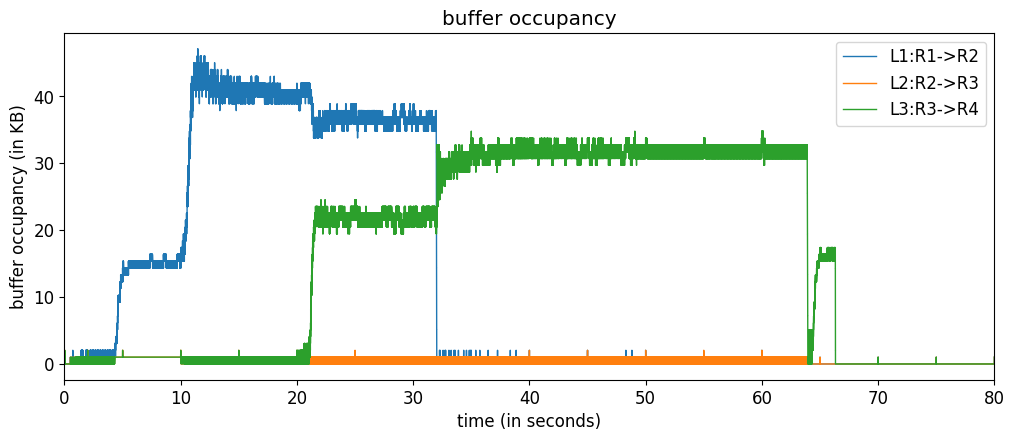
\includegraphics[width = \textwidth]{test_case2_fast buffer occupancy.png}
\end{figure}

The buffer occupancy that we observe on all our links can be explained by a couple different things. First, when we just have one flow, we know that only the buffer for link one is going to be used. We can see that this buffer has an occupancy of 15, because our alpha parameter for our flows is 15 which represents the amount of packets that flow 1 has in buffers along its route. 

At 10 seconds, when flow 2 is added, our buffer's occupancy rises to ~45. This is incremented by 30 instead of 15 like one could expect, because when our second flow starts sending packets, its initial rtt min calculation is one where there are already 15 packets in the buffer. This means in the window size equation it adjusts its window assuming there are 0 packets in a link where there is actually 15. Thus, it can have 30 packets in buffers along its path instead of 15, which is why link one will have 45 packets in its buffer when both flow 1 and flow 2 are going.

When our third flow is started, it tries to add 15 packets to its bottleneck as well. However, there are still packets from flow one that flow three uses in its calculation of the min rtt. This means that flow three will add 15 packets to the third buffer, but some more packets are added to the buffer by flow 1. Flow 1 adds a total of 15 packets to buffer 1 and buffer 3, which is split between the two of them (as seen in our graphs)

Then, once flow two finishes, flow 1 and flow 3 are sharing L3, and as expected, 30 packets are queued in the buffer, which corresponds to 15 for each flow.

Once flow 1 finishes, we can see that flow 3 needs time to start sending packets faster to fill the buffer at all, which is why we get a large drop of buffer occupancy immediately after flow one finishes.

\begin{figure}[H]
\centering
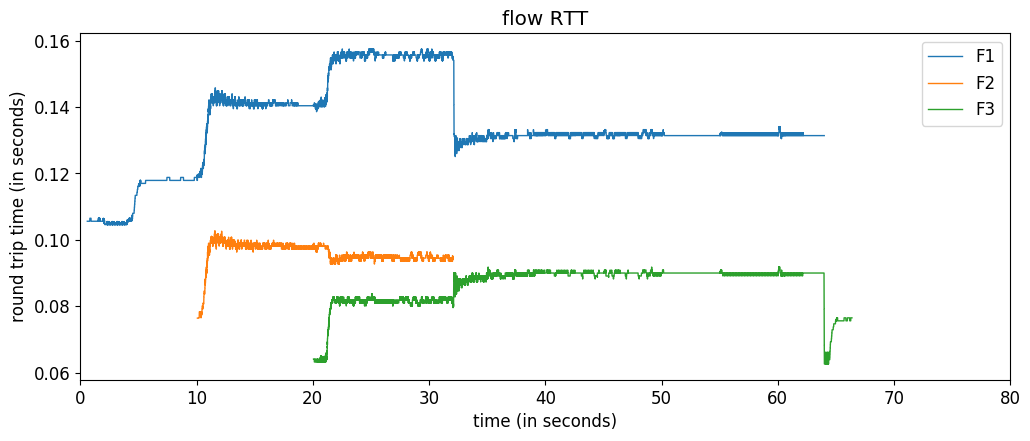
\includegraphics[width = \textwidth]{test_case2_fast flow RTT.png}
\end{figure}

We can see that our round trip times are very closely correlated to how full our buffers are, because the more full that our buffers are, the longer each packet has to spend in the link queue and thus will have longer queuing delays.

\begin{figure}[H]
\centering
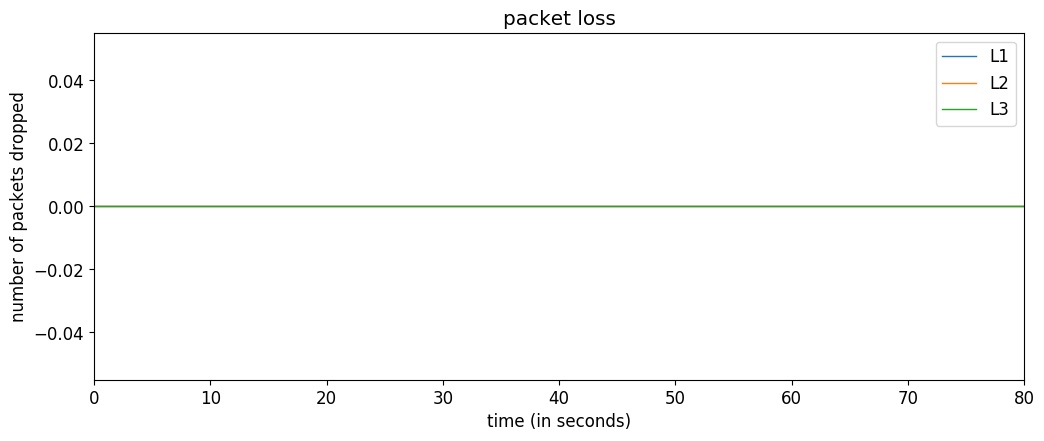
\includegraphics[width = \textwidth]{test_case2_fast packet loss.png}
\end{figure}

This is expected behavior because we do not lose any packets using fast.



\subsection{Test Case 3} 

Run using \textbf{python3 main.py test\_case3.json 20}.

\begin{figure}[H]
\centering
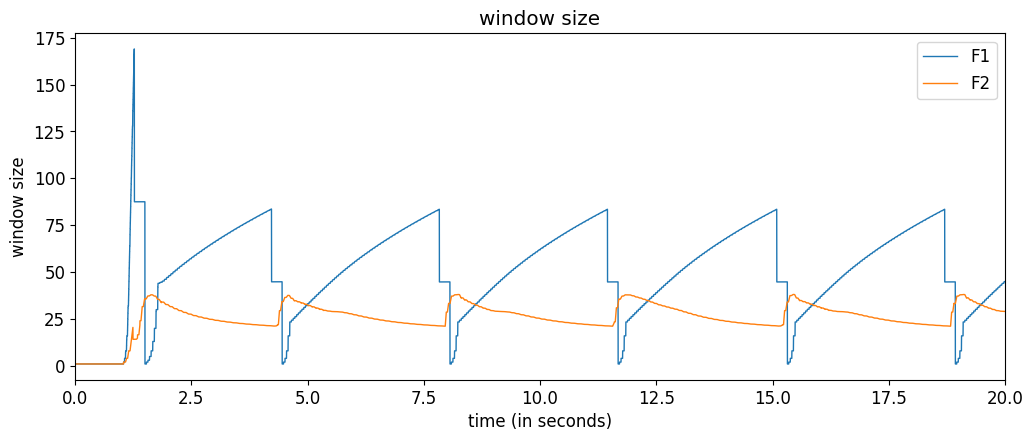
\includegraphics[width = \textwidth]{test_case3 window size.png}
\end{figure}

\begin{figure}[H]
\centering
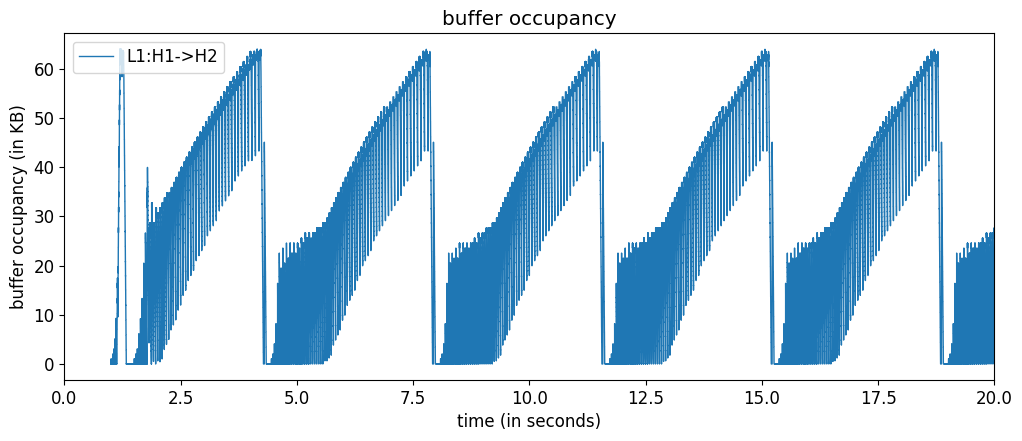
\includegraphics[width = \textwidth]{test_case3 buffer occupancy.png}
\end{figure}

\begin{figure}[H]
\centering
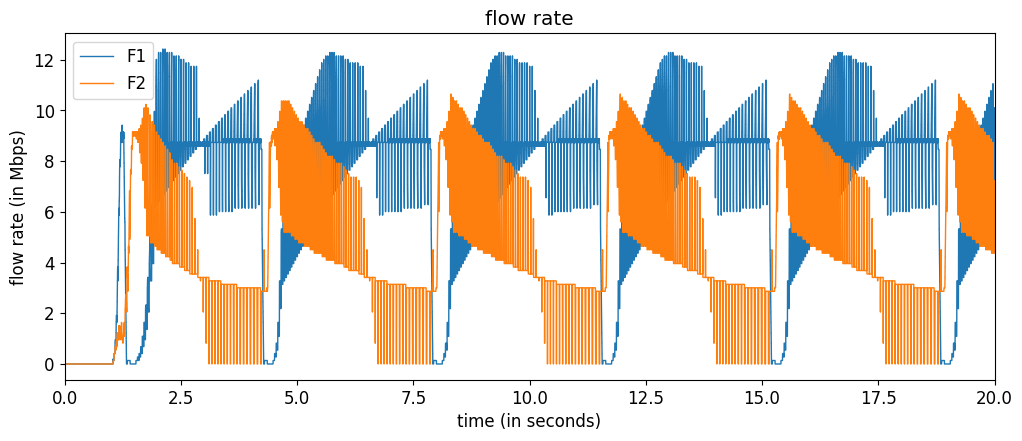
\includegraphics[width = \textwidth]{test_case3 flow rate.png}
\end{figure}

\begin{figure}[H]
\centering
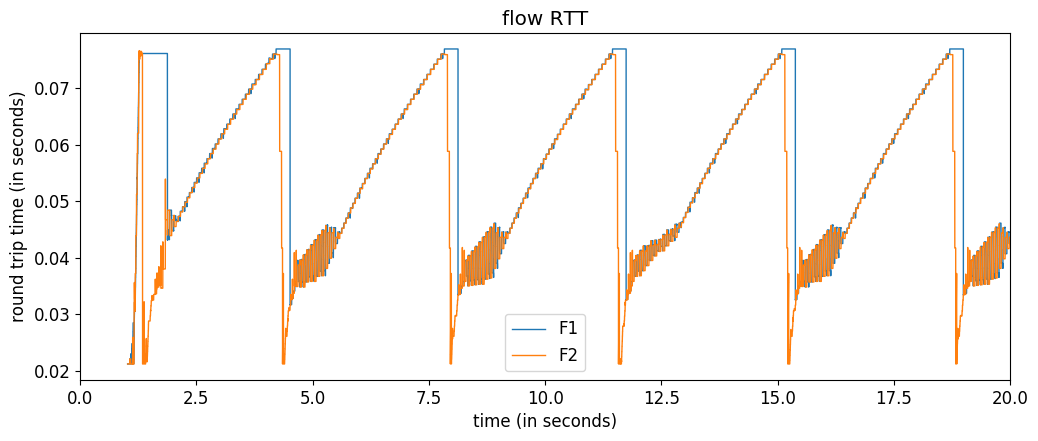
\includegraphics[width = \textwidth]{test_case3 flow RTT.png}
\end{figure}

\begin{figure}[H]
\centering
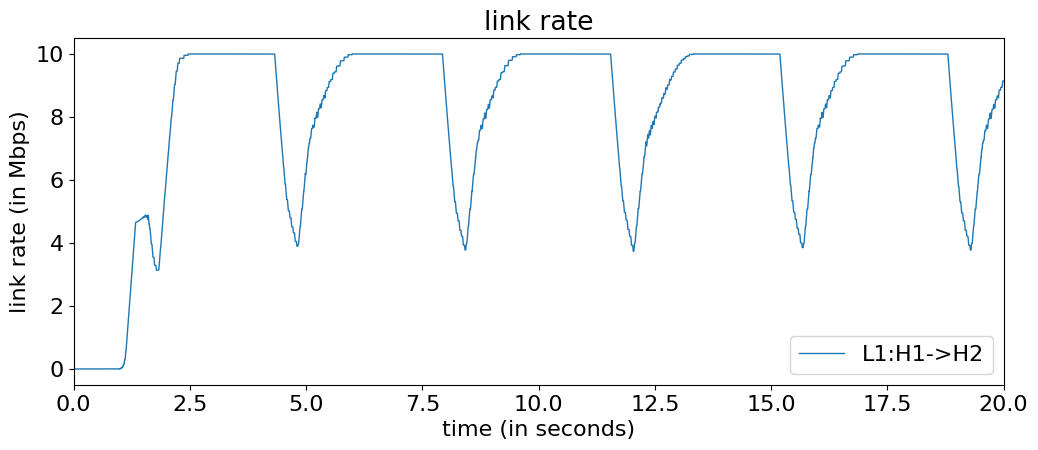
\includegraphics[width = \textwidth]{test_case3 link rate.png}
\end{figure}

\begin{figure}[H]
\centering
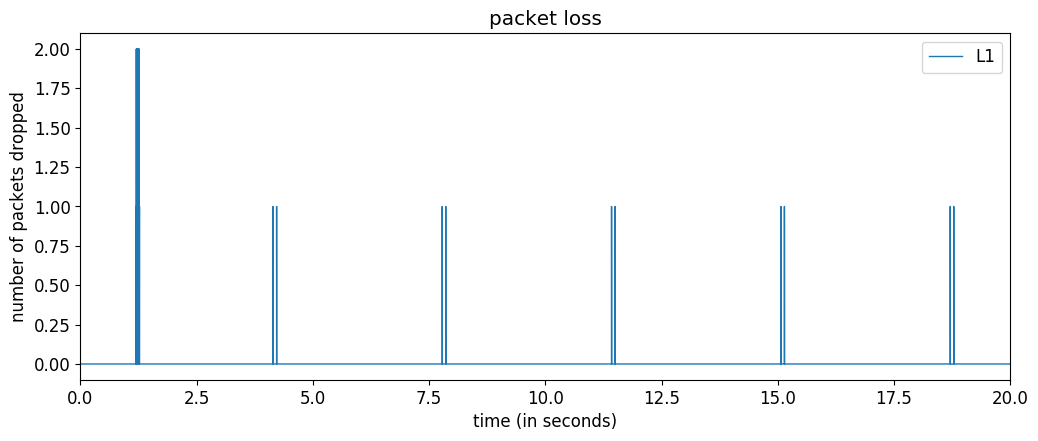
\includegraphics[width = \textwidth]{test_case3 packet loss.png}
\end{figure}


\subsection{Test Case 4}

Run using \textbf{python3 main.py test\_case4.json 20}.

\begin{figure}[H]
\centering
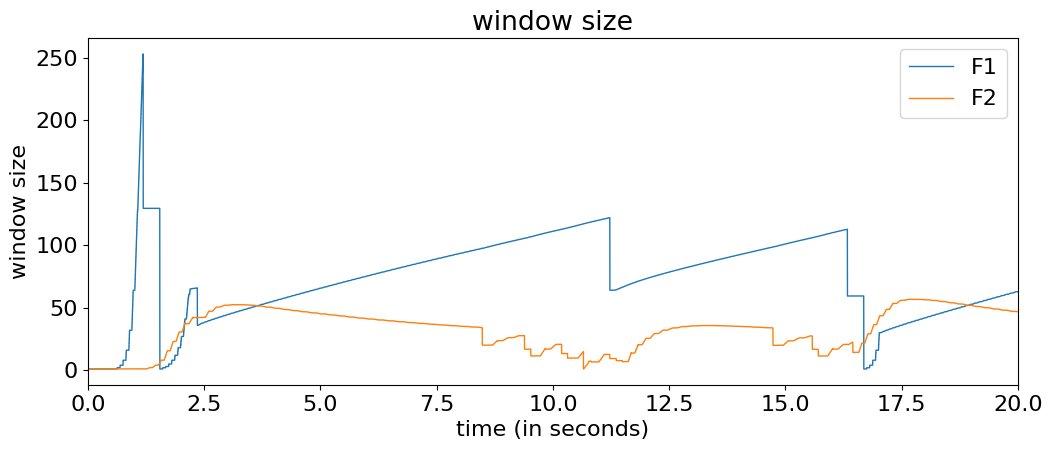
\includegraphics[width = \textwidth]{test_case4 window size.png}
\end{figure}

Initially, we see both the explosion from Reno and the slow start into congestion avoidance from FAST. As Flow 1 gets faster, Flow 2 anticipates dropping packets and backs off, only giving Flow 1 more space to grow until eventually entering fast recovery around 11.25 seconds. Flow 2 experiences a strange result. It continuously drops packets and enters fast recovery and congestion avoidance, even timing out once. This is again only explained by the way link priority works in our system, which was not intentional. Our implementation fires off each link one at a time every time increment. In this case, based on how we created our links, L1 has priority over L2; L1 sends packets before L2 at a given time increment. Thus, Flow 2 is more likely to drop packets and react, while Flow 1 can expand and dominate Flow 2. This is an unfortunate result due to our implementation but it was not evident until the final week. As you can see, given this explanation, everything works as it would, and when Flow 1 times out completely, Flow 2 gains more space to increase its window size before having to adjust once more.

\begin{figure}[H]
\centering
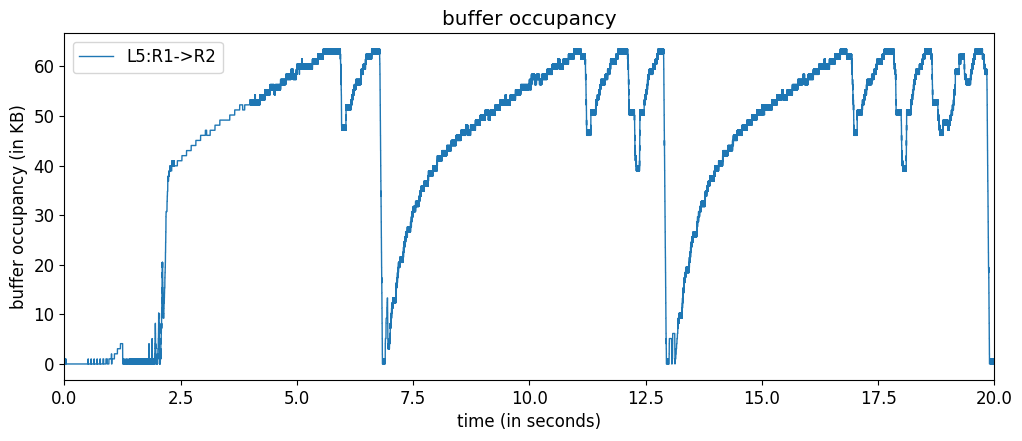
\includegraphics[width = \textwidth]{test_case4 buffer occupancy.png}
\end{figure}

The buffer occupancy closely mirrors the two window sizes. When Flow 1, which is the most dominant flow, experiences fast recovery, the buffer almost completely clears out, but then quickly fills up again as the flow continues with its congestion avoidance.

\begin{figure}[H]
\centering
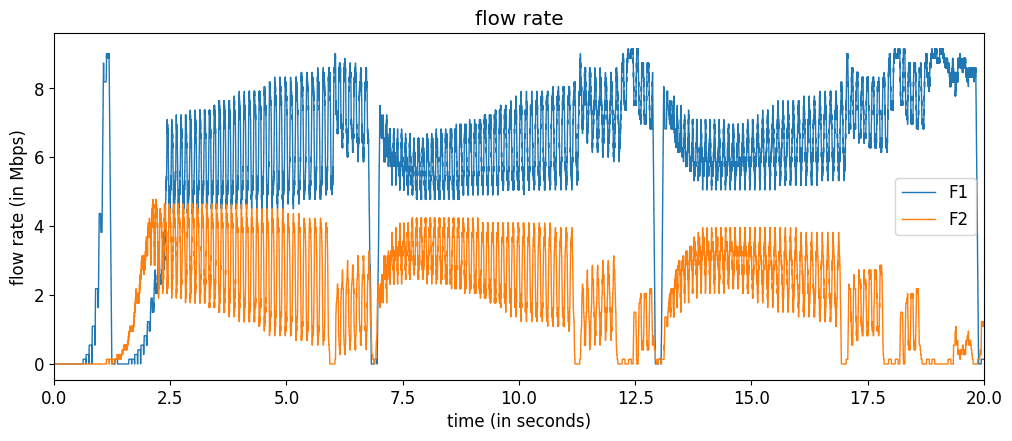
\includegraphics[width = \textwidth]{test_case4 flow rate.png}
\end{figure}

The flow rate also closely mirrors window size, becoming zero around the same times as the fast recovery and timeouts occur. In general, Flow 1 is dominant and aggressive and dominates the flow rate competition, minimizing FAST's flow rate, except when Flow 1 times out and Flow 2 has an opportunity to increase its flow rate, only to come down once more.

\begin{figure}[H]
\centering
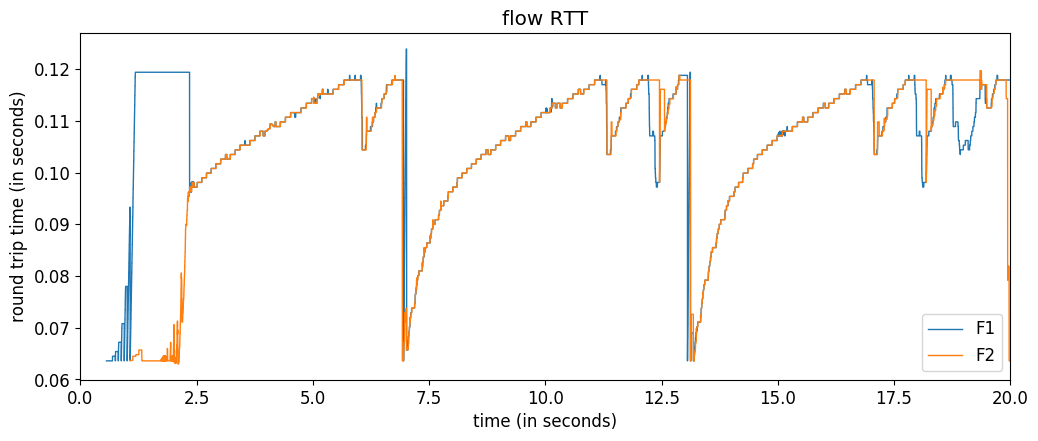
\includegraphics[width = \textwidth]{test_case4 flow RTT.png}
\end{figure}

Flow RTT very closely mirrors the buffer occupancy, which makes sense as in general the propagation delay remains the same and the queueing delay changes. The few times that the F2 flow RTT remains constant is because we are in fast recovery and we do not update our RTT in this case given Karn's algorithm.

\begin{figure}[H]
\centering
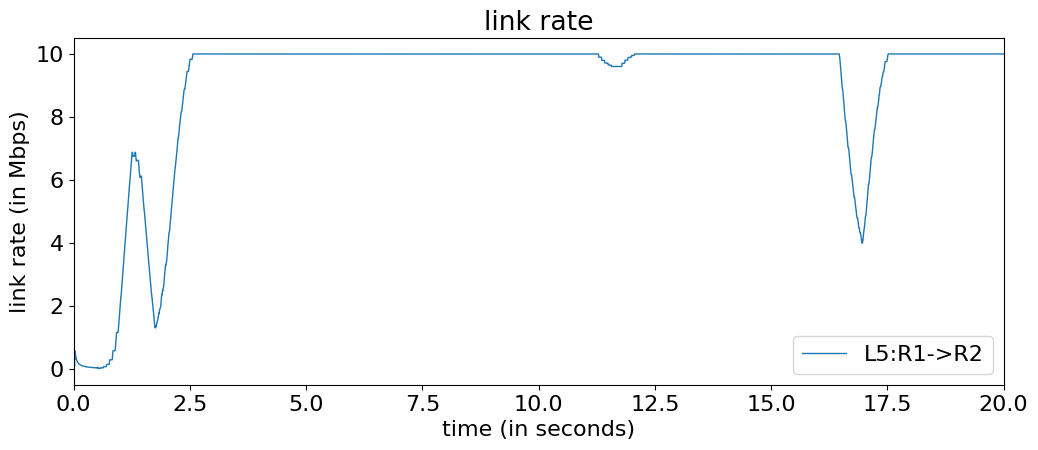
\includegraphics[width = \textwidth]{test_case4 link rate.png}
\end{figure}

Link rate is as we would expect. Mostly constant with a big drop when Flow 1 times out.

\begin{figure}[H]
\centering
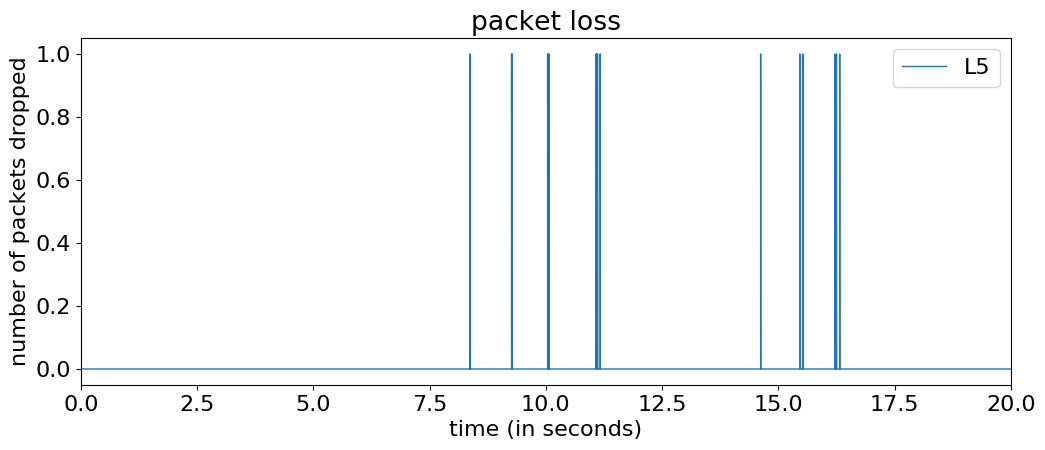
\includegraphics[width = \textwidth]{test_case4 packet loss.png}
\end{figure}

Packet loss correlates with buffer occupancy reaches 64 as expected.



\subsection{Test Case 5}

\subsubsection{TCP Reno}

Run using \textbf{python3 main.py test\_case5\_reno.json 20}.

\begin{figure}[H]
\centering
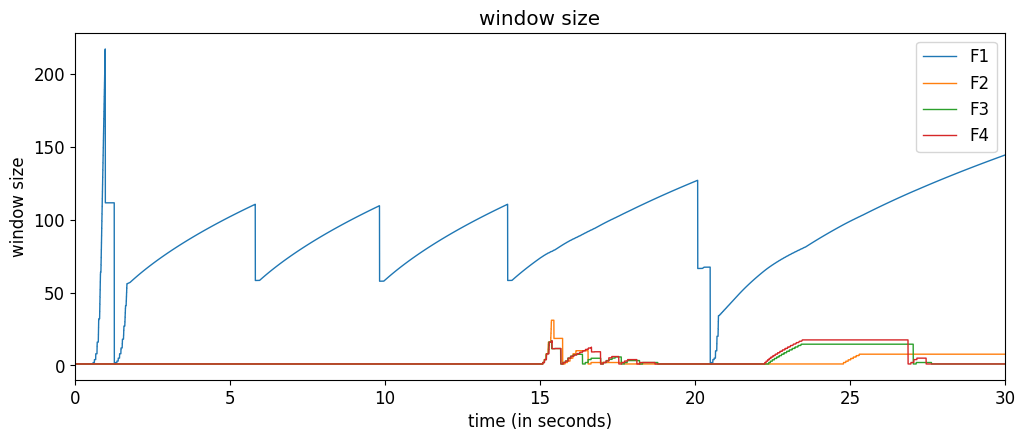
\includegraphics[width = \textwidth]{test_case5_reno window size.png}
\end{figure}

We see that the dominant flow in this graph is F1, which makes sense since it starts at 0.5s. So for 14.5 s, this is the only flow moving through L5, allowing it to dominate the link capacity. While the flows sends packets as the only flow in the network, we see classic TCP Reno behavior. We have a slow start, where the window size increases dramatically, until we have a dropped packet and halve our window size. Then, we have a packet timeout, which causes us to re-enter slow start with a new threshold, after which we enter congestion avoidance. We then stabilize into a pattern of congestion avoidance and FRFR when a packet is dropped.

However, at about 15 s, we see the other flows in the network start up. But the peaks of their slow start states is significantly smaller since they must share the network with the other flows. Moreover, our links are built with an inherent priority in terms the order links have their packets processed by the router and then added to the buffer of L5. This is especially evident in this graph, since the router prioritizes packets from L1 then L2 then L3 and then L4, so it's more likely that packets from L4 are dropped more frequently because by the time R1 processes them, the buffer of L5 is already full. As the packets from L2, L3, and L4 get dropped, we see that the corresponding flows repeatedly enter congestion avoidance and timing out. So, we see these flows have all timed outs and are waiting until 23 s to start sending again.

We also see a packet timeout at around L5, and this results in F1 re-entering slow start, as a result of it exceeding its threshold. This behavior is surprising, since we expected to see a continuation of the sawtooth pattern. 

\begin{figure}[H]
\centering
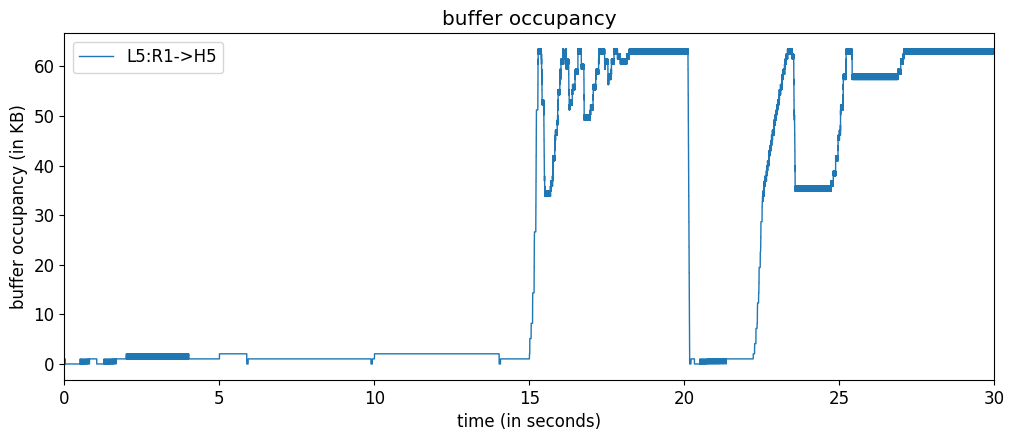
\includegraphics[width = \textwidth]{test_case5_reno buffer occupancy.png}
\end{figure}

A major feature of this graph is massive spike in buffer occupancy at around 15 s when all of the remaining flows start. This makes sense as all packets from all flows are trying to access L5. Moreover, we see a large dropoff at 20s, when we enter a timeout and stop sending packets until our retransmission is successful. 

\begin{figure}[H]
\centering
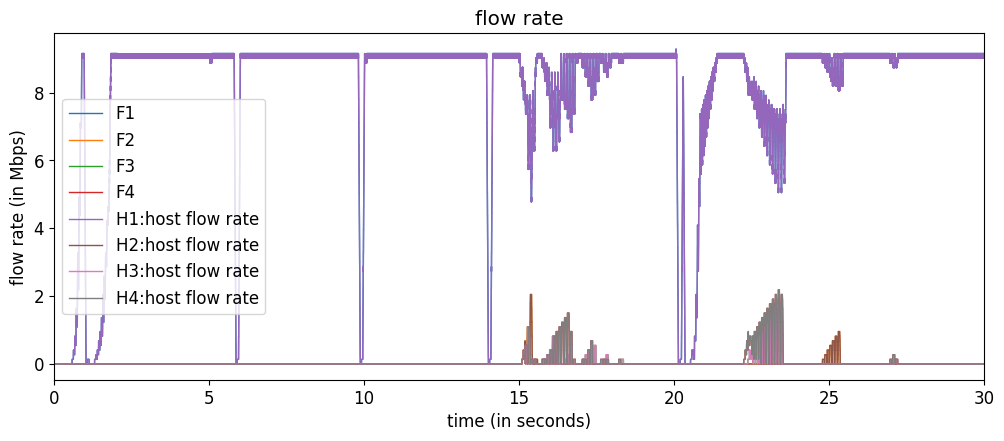
\includegraphics[width = \textwidth]{test_case5_reno flow rate.png}
\end{figure}

We see our total flow rate remains consistent throughout the simulation. We see that the drops in flow rate in the first 15s correspond to when the simulator enters CA. Afterwards, we see the flow rate of F0 occasionally decreases as it makes way for other flows to send their packets.

\begin{figure}[H]
\centering
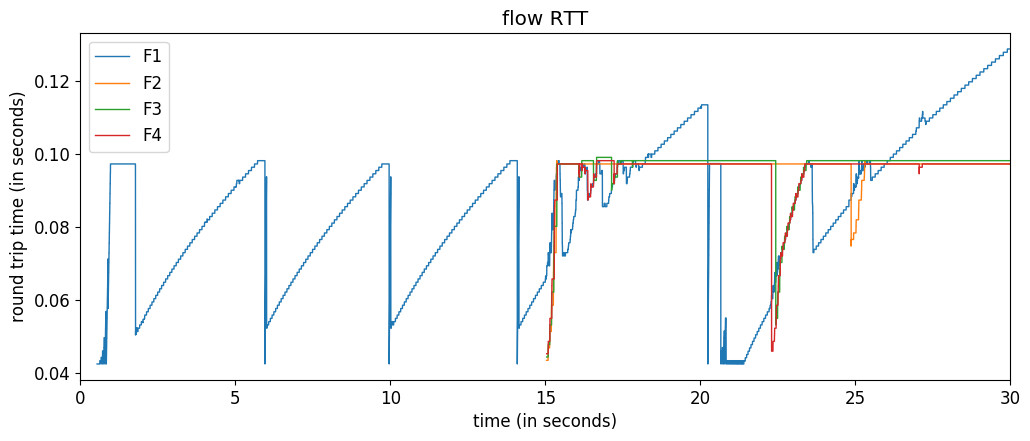
\includegraphics[width = \textwidth]{test_case5_reno flow RTT.png}
\end{figure}

The flow RTT is consistent with what we'd expect TCP Reno to look like for F1 for the first 15s. However, the behavior of the RTT then increasing for every sawtooth pattern afterwards is unexpected. The other flows have very similar RTT graphs to each other as expected as they have the same properties.

\begin{figure}[H]
\centering
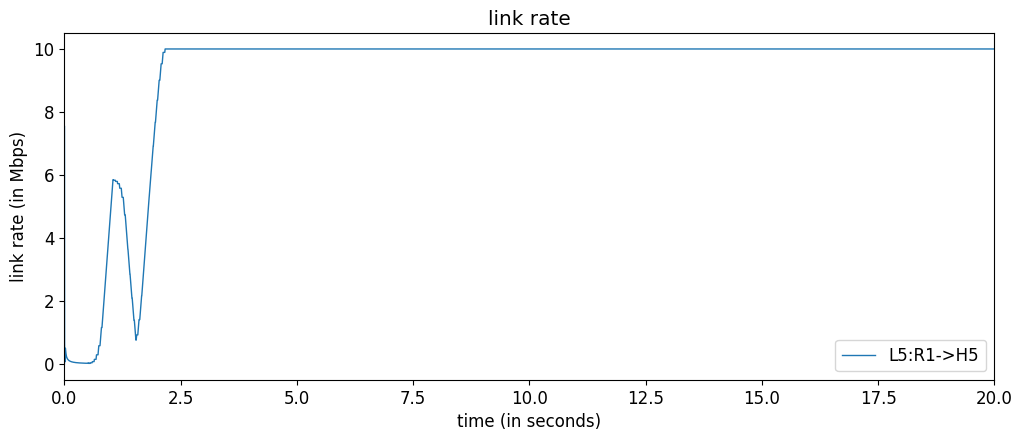
\includegraphics[width = \textwidth]{test_case5_reno link rate.png}
\end{figure}


The link rate graph has dips that match when F1 enters FRFR and congestion avoidance. Moreover, it contains one large dip at 20s which matches when F1 times out and F2, F3< and F4 are waiting for their timeouts to end, and no packets are being sent at all.

\begin{figure}[H]
\centering
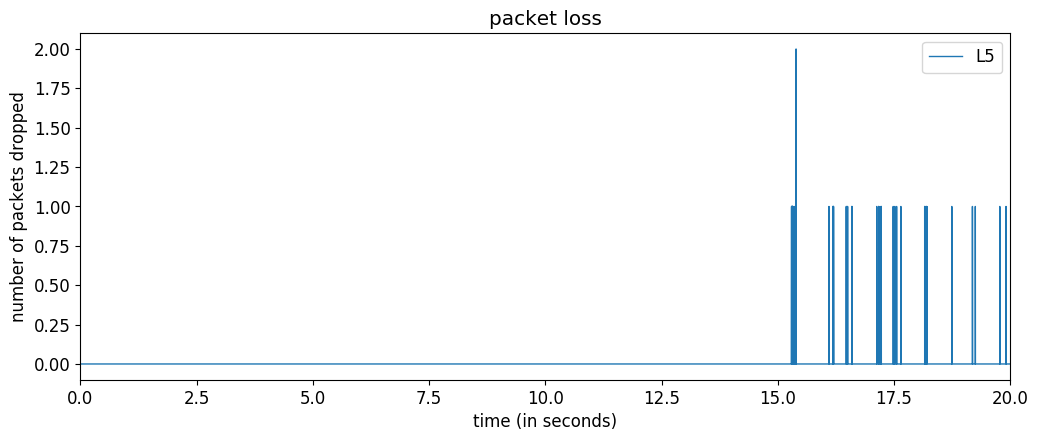
\includegraphics[width = \textwidth]{test_case5_reno packet loss.png}
\end{figure}


Our packet loss graph has a few notable traits, specifically the number of losses at around 15s. This occurs because as flows 2, 3, and 4 start at 15 s, all of the hosts send their packets to R1. Once R1 receives these packets, it tries to add them to the buffer of L5 to send them to H5. However, the buffer quickly fills, and as a result packets are dropped. We note that this pattern repeats afterwards as the packets timeout for F2, F3, F4 after the previous timeout ends.

\subsubsection{TCP Fast}

Run using \textbf{python3 main.py test\_case5\_fast.json 20}.

\begin{figure}[H]
\centering
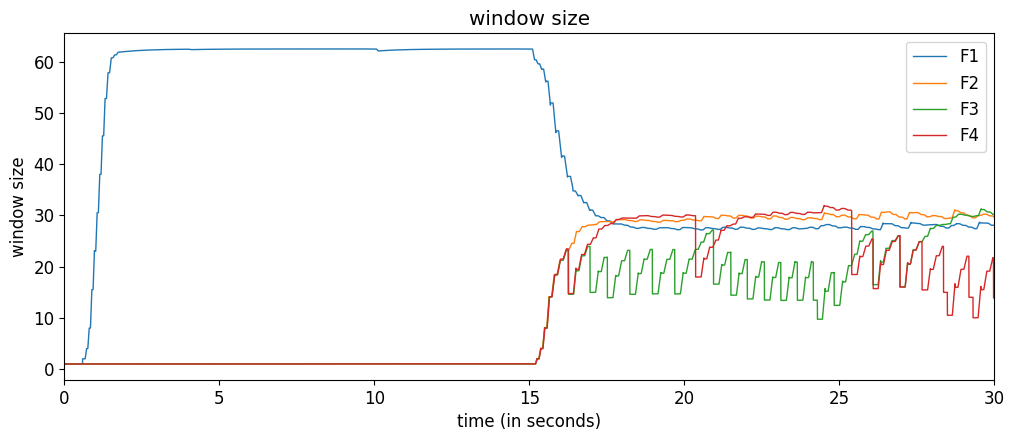
\includegraphics[width = \textwidth]{test_case5_fast window size.png}
\end{figure}


The window size graph has a couple notable traits. First, initially our first flow which is alone goes into slow start and reaches an equilibrium state in congestion avoidance. Then, once all of our other flows start at 15 seconds, they all go into slow start and get to their congestion avoidance phase. 

The expected behavior is that all 4 flows should have a comparable window size to each other once equilibrium is hit. However, this is not the case, as we can see Flow 3 does not ever reach that equilibrium point. This can be explained by the priorities that occur within our links, and the fact that when we have all 4 flows packets being sent together, flow 3's packets are dropped. When flow 3 drops packets, it goes into FRFR state until it steadies, and then back into congestion avoidance. The buffer for link 5 is already full with the occupancy of the three other flows, and then when flow 3 tries to increase its window size to equilibrium, since it is connected to the last link that is sending its packets, it will not be able to send its packets after a certain point, and thus another packet will be dropped and flow 3 will revert back to its FRFR state. 

\begin{figure}[H]
\centering
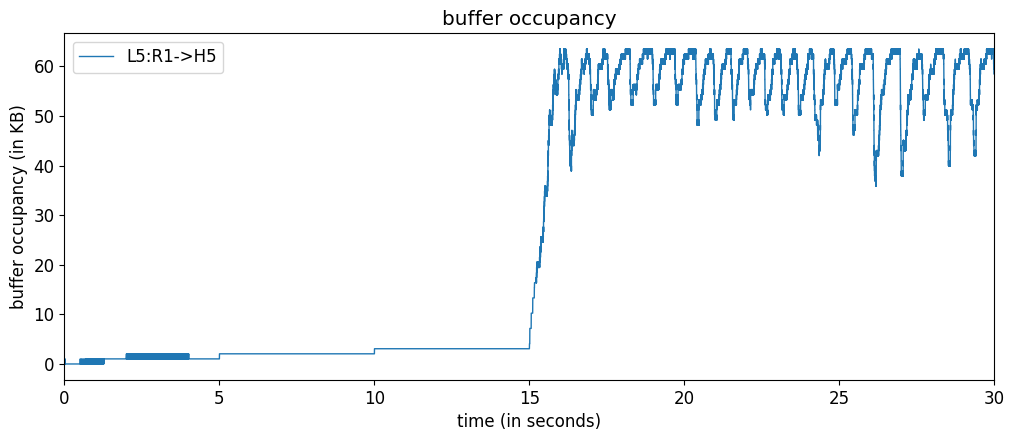
\includegraphics[width = \textwidth]{test_case5_fast buffer occupancy.png}
\end{figure}

Our buffer occupancy can easily be explained by the behavior of all of our flows. We can see that our buffer tries to have 15 packets per flow in it at all times, but when one flow (flow 3) drops its packets, its window size will drop and is unable to add 15 packets at certain points. This then causes our buffer occupancy to drop suddenly, because flow 3 is will be adding less packets to the buffer than expected.

\begin{figure}[H]
\centering
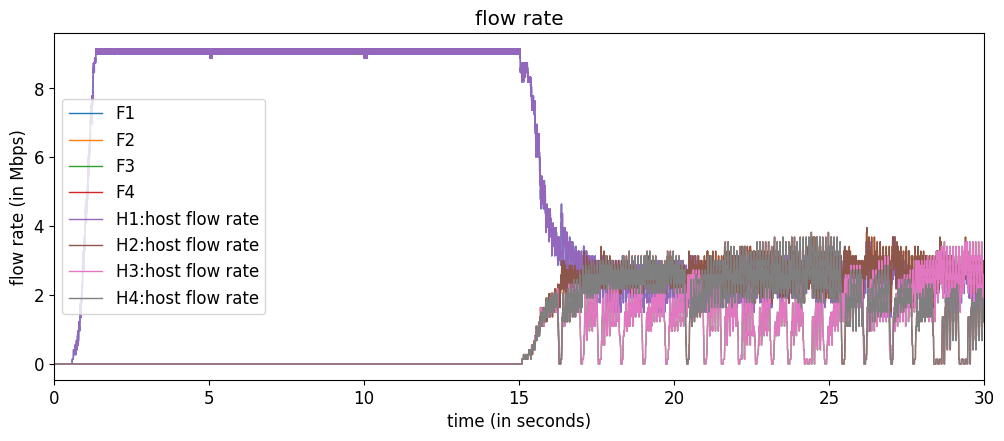
\includegraphics[width = \textwidth]{test_case5_fast flow rate.png}
\end{figure}

The flow rate graph can be explained with similar logic as our other graphs. We can see that the flow rate is dependent on the window size of each of our flows. Since we know that flow 3 never reaches equilibrium in its congestion avoidance stage, it is clear that when it continually drops packets, its flow rate cannot reach equilibrium. However, since none of the other flows are dropping any packets, it makes sense for them all to have the same equilibrium state and flow rate as each other, which is sharing the rate of link 5.

\begin{figure}[H]
\centering
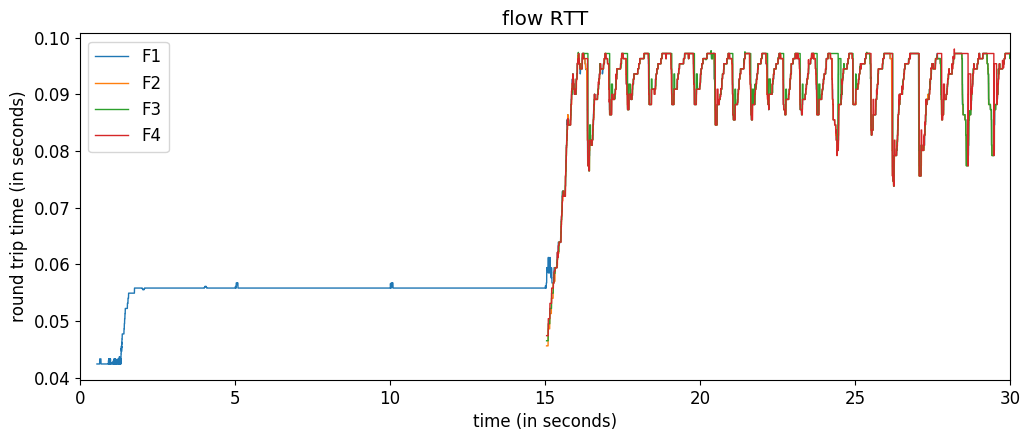
\includegraphics[width = \textwidth]{test_case5_fast flow RTT.png}
\end{figure}

Our round trip times are easily modeled by our buffer occupancy. Clearly, packets take more time to send when there is more information in each of the buffers because the packet will have more queuing delay. Thus, our RTT time mirrors our buffer occupancy.

\begin{figure}[H]
\centering
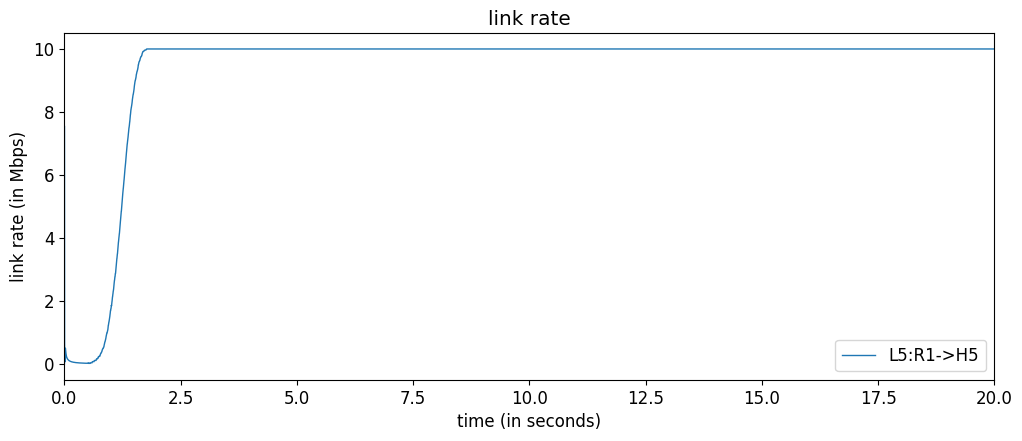
\includegraphics[width = \textwidth]{test_case5_fast link rate.png}
\end{figure}


Our link rate makes sense, because once our first flow starts using the link, it should be consistently full because it is always the bottlenecked link.

\begin{figure}[H]
\centering
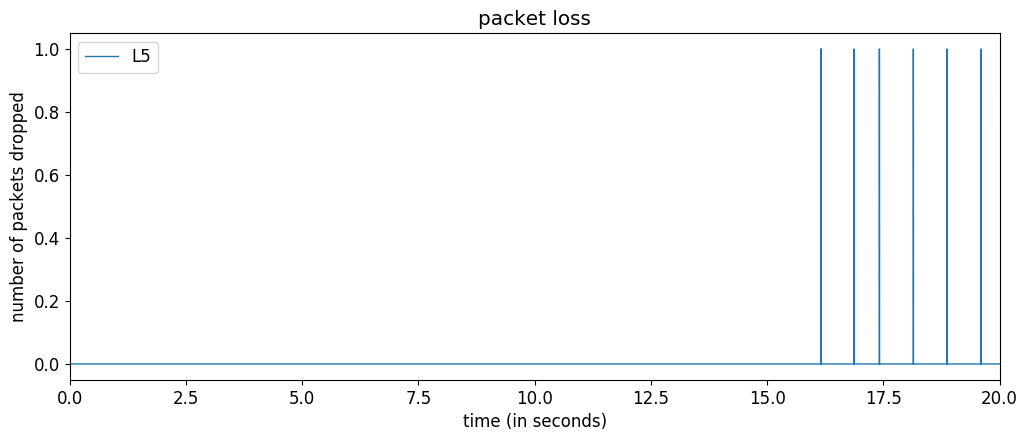
\includegraphics[width = \textwidth]{test_case5_fast packet loss.png}
\end{figure}

We lose packets once we are sending multiple different flows down one link (4). These packets are lost in our flow 3 going into FRFR stages as they are trying to reach equilibrium but cannot because the buffer becomes full from the other flows because the other flows are prioritized in the algorithm that we use.


\subsection{Our Test Case}

Run using \textbf{python3 main.py test\_case\_custom.json 20}.

\begin{figure}[H]
\centering
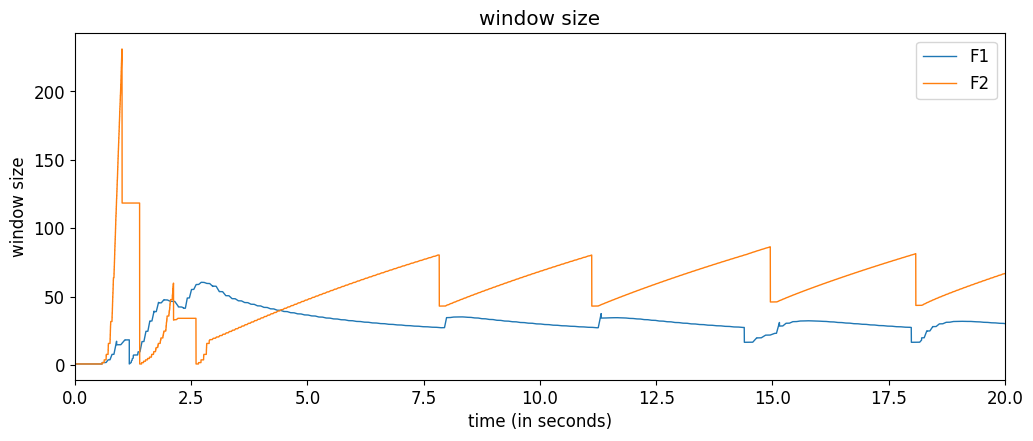
\includegraphics[width = \textwidth]{test_case_custom window size.png}
\end{figure}

\begin{figure}[H]
\centering
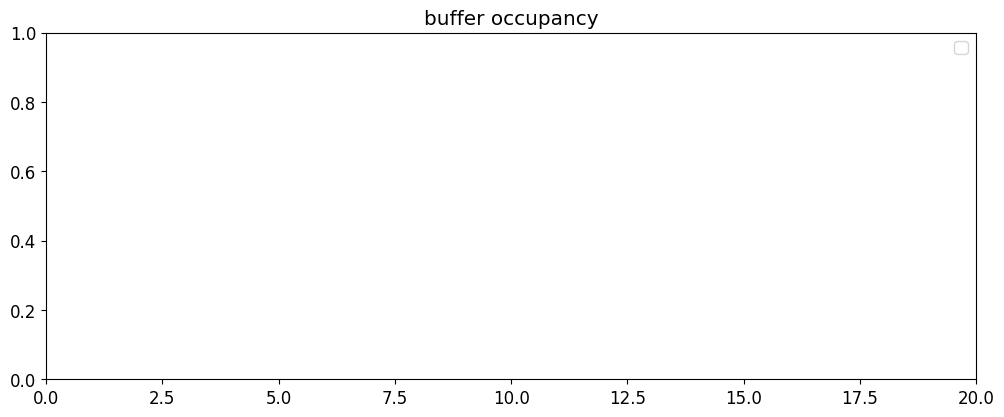
\includegraphics[width = \textwidth]{test_case_custom buffer occupancy.png}
\end{figure}

\begin{figure}[H]
\centering
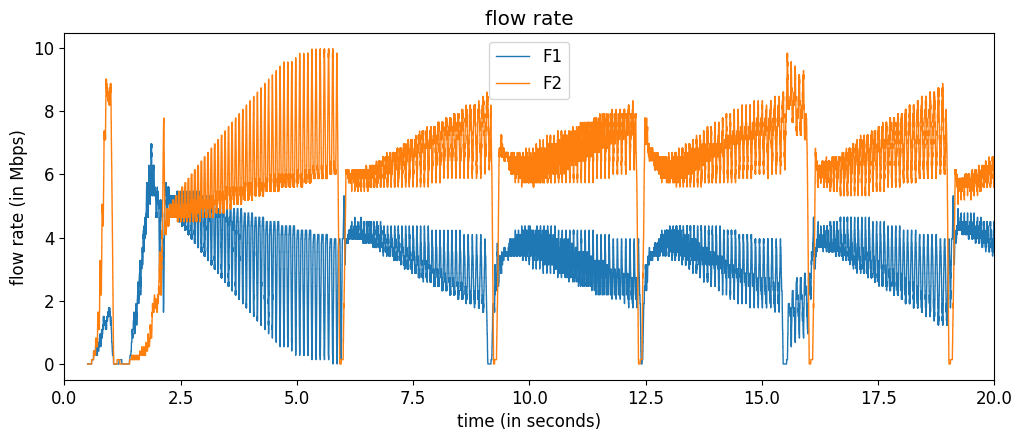
\includegraphics[width = \textwidth]{test_case_custom flow rate.png}
\end{figure}

\begin{figure}[H]
\centering
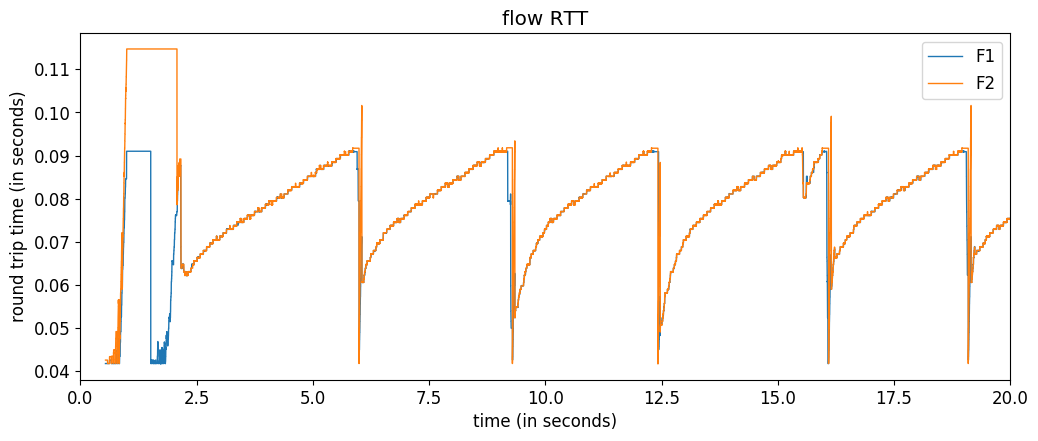
\includegraphics[width = \textwidth]{test_case_custom flow RTT.png}
\end{figure}

\begin{figure}[H]
\centering
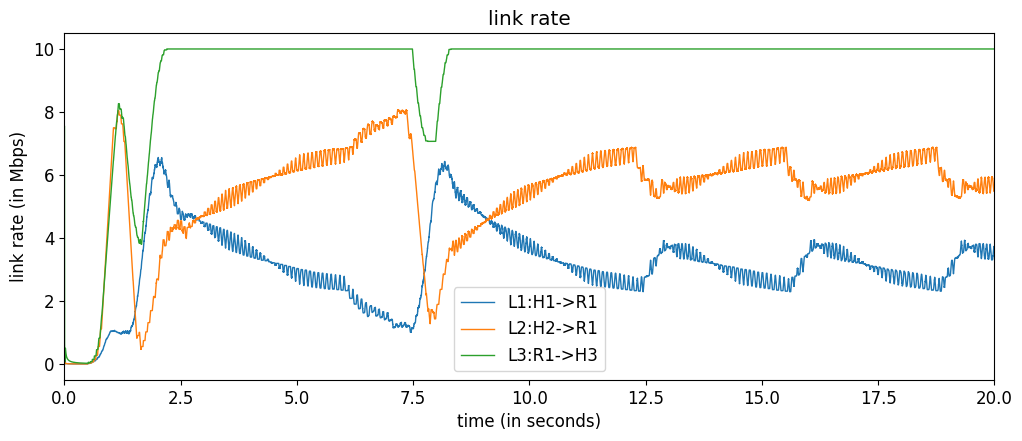
\includegraphics[width = \textwidth]{test_case_custom link rate.png}
\end{figure}

\begin{figure}[H]
\centering
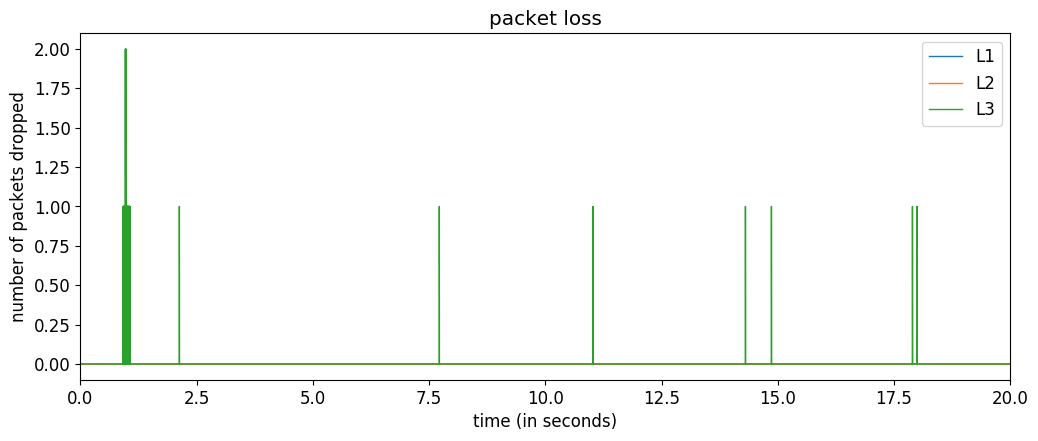
\includegraphics[width = \textwidth]{test_case_custom packet loss.png}
\end{figure}


\section{Timeline \& Division of Labor}

\subsection{Timeline}

\begin{description}
  \item[$\bullet$ Weeks 4-6:] Completed initial architecture design of simulator and initial implementation of a few simulator classes, such as Packet and Link classes
  \item[$\bullet$ Weeks 7-8:] Completed initial implementation of all class in the simulator, started debugging Router and Flow classes 
  \item[$\bullet$ Week 9:] Finished debugging fundamental architecture for simulator, started work on implementing and debugging TCP Reno congestion control
  \item[$\bullet$ Week 10:] Finished implementation of TCP Reno Congestion Control, debugging metric tracking
  \item[$\bullet$ Week 11:] Finished implementation of TCP Fast, finished report and presentation
\end{description}

\subsection{Division of Labor}

\begin{description}
    \item[$\bullet$ Everyone:] Initial architecture design, report \& presentation slides
	\item[$\bullet$ Rafael Fueyo-Gomez:] Hosts, routers, flow, congestion control (TCP Reno and TCP Fast)
	\item[$\bullet$ Cortland Perry:] Routers, congestion control (TCP Fast)
	\item[$\bullet$ Kelsi Riley:] Links, initial implementation, metric tracking, congestion control (TCP Fast)
	\item[$\bullet$ Sakthi Vetrivel:] Flows, congestion control (TCP Reno) 
\end{description}

\end{document}